\documentclass[tikz,border=6pt]{standalone}
\usepackage{tikz}
\begin{document}
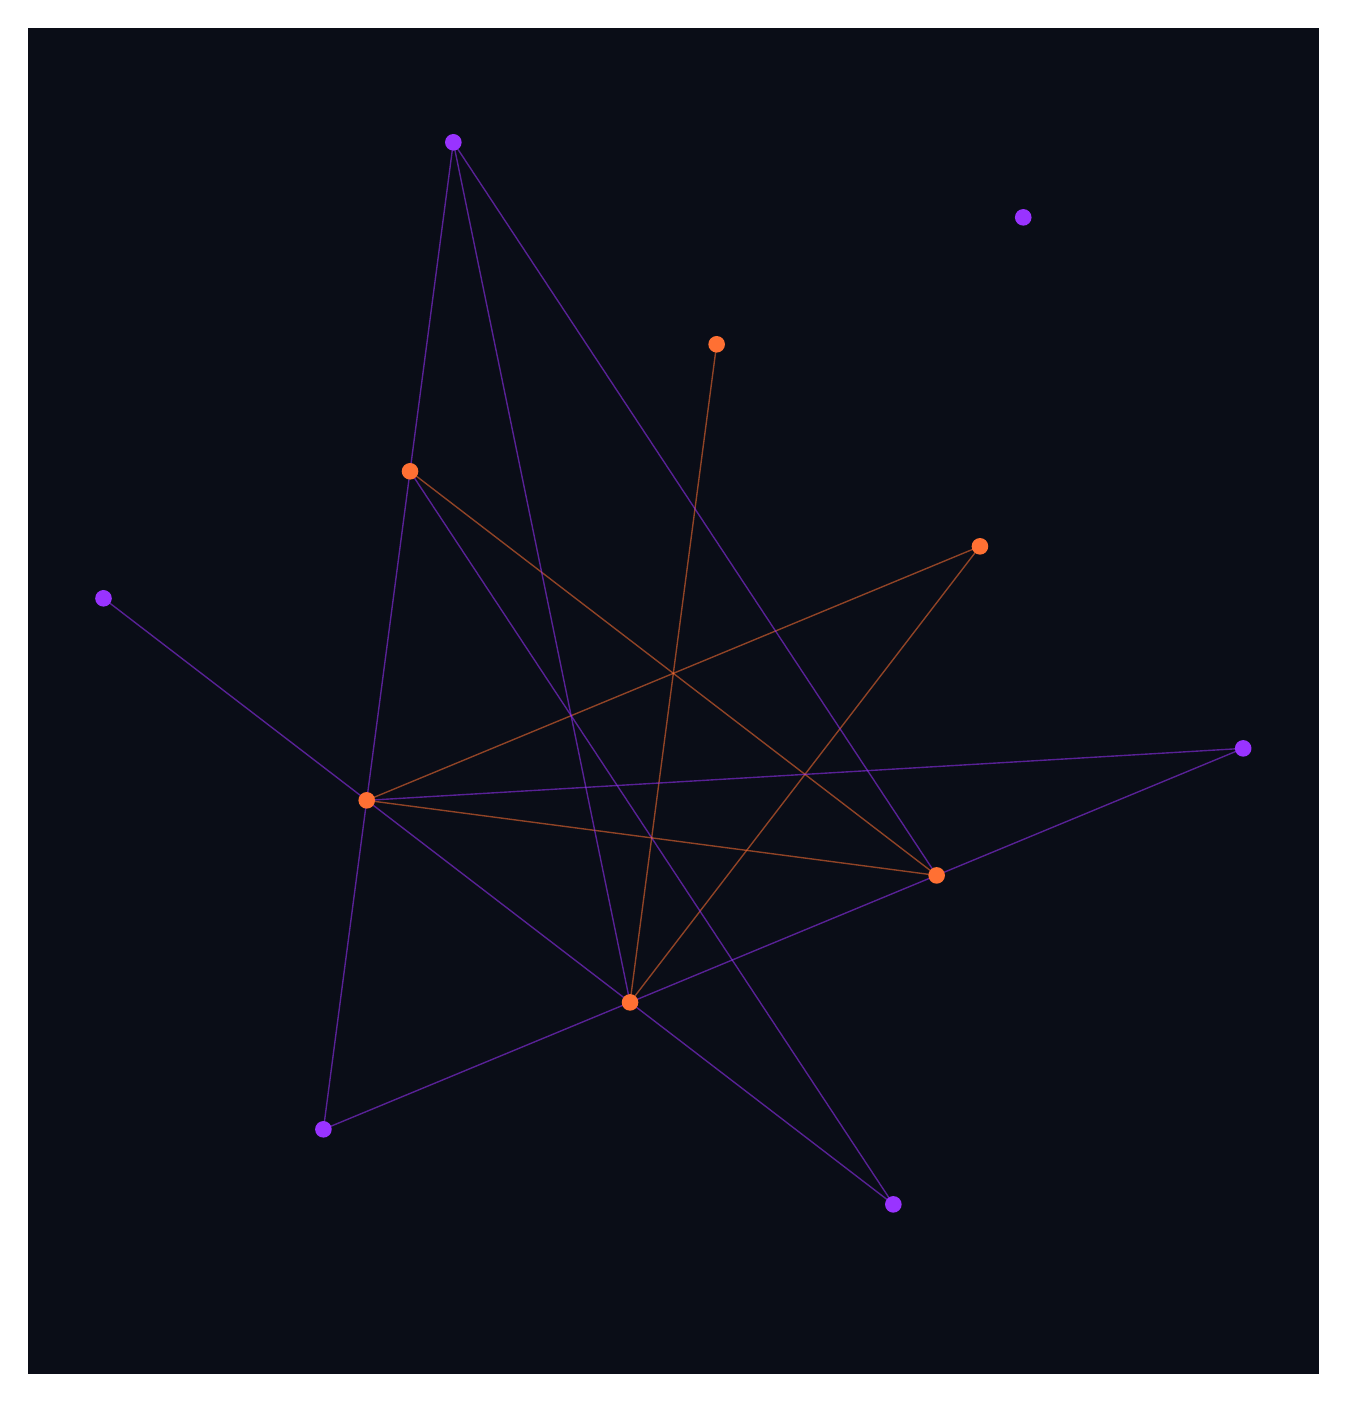
\begin{tikzpicture}
\definecolor{ring0}{rgb}{1.000,0.440,0.200}
\definecolor{ring1}{rgb}{0.600,0.200,1.000}
\definecolor{bg}{rgb}{0.04,0.05,0.09}
\fill[bg] (-8.2,-8.9) rectangle (8.2,8.2);
\draw[ring0,line width=0.5pt,opacity=0.55] (3.894,1.613)--(-3.894,-1.613);
\draw[ring0,line width=0.5pt,opacity=0.55] (3.894,1.613)--(-0.550,-4.179);
\draw[ring0,line width=0.5pt,opacity=0.55] (0.550,4.179)--(-0.550,-4.179);
\draw[ring0,line width=0.5pt,opacity=0.55] (-3.344,2.566)--(3.344,-2.566);
\draw[ring1,line width=0.5pt,opacity=0.55] (-3.344,2.566)--(2.794,-6.744);
\draw[ring0,line width=0.5pt,opacity=0.55] (-3.894,-1.613)--(3.344,-2.566);
\draw[ring1,line width=0.5pt,opacity=0.55] (-3.894,-1.613)--(7.237,-0.953);
\draw[ring1,line width=0.5pt,opacity=0.55] (-0.550,-4.179)--(-2.794,6.744);
\draw[ring1,line width=0.5pt,opacity=0.55] (3.344,-2.566)--(-2.794,6.744);
\draw[ring1,line width=0.5pt,opacity=0.55] (-2.794,6.744)--(-4.444,-5.791);
\draw[ring1,line width=0.5pt,opacity=0.55] (-7.237,0.953)--(2.794,-6.744);
\draw[ring1,line width=0.5pt,opacity=0.55] (-4.444,-5.791)--(7.237,-0.953);
\fill[ring0] (3.894,1.613) circle (3.0pt);
\fill[ring0] (0.550,4.179) circle (3.0pt);
\fill[ring0] (-3.344,2.566) circle (3.0pt);
\fill[ring0] (-3.894,-1.613) circle (3.0pt);
\fill[ring0] (-0.550,-4.179) circle (3.0pt);
\fill[ring0] (3.344,-2.566) circle (3.0pt);
\fill[ring1] (4.444,5.791) circle (3.0pt);
\fill[ring1] (-2.794,6.744) circle (3.0pt);
\fill[ring1] (-7.237,0.953) circle (3.0pt);
\fill[ring1] (-4.444,-5.791) circle (3.0pt);
\fill[ring1] (2.794,-6.744) circle (3.0pt);
\fill[ring1] (7.237,-0.953) circle (3.0pt);
\end{tikzpicture}
\end{document}